\section{Diskussion}
Bei dem Vergleich von \textsc{MiniDogNN} mit den vortranierten Modellen,
zeigt sich deutlich, welchen Einfluss die FCN auf die Genauigkeiten der
Klassifizier haben. Die Genauigkeit ist somit deutlich mit der Anzahl an Features
die das FCN klasssifiziert korreliert. Desweiteren zeigt sich bei \textsc{MiniDoggNN}-Architektur
für $120$ Rassen, dass die Anzahl der Neuronen pro Lage eine geringe Anzahl an
Features scheinbar nicht ausgleichen kann.

Die Verwendung eines AutoEncoders und eines RF hat für $5$ Hunderassen bereiteis
eine schlechtere Performance, als die zugehörige \textsc{MiniDogNN}-Architektur.
Die schlechte Genaugkeit, ist vermutlich auf die geringe Bildgöße von $96\times96$
zurückzuführen. Ein Eigenschaft die, wie getestet, selbst der \textsc{PreDogNN}-Architektur
die Klassifizierung erschwert und die Genauigkeit auf $60\%$. Diese Abhäbgigkeit
lässt sich auf die Informationsreduzierung bei Runterskalierung zurückführen.

Die durchgeführt HPO für das \textsc{MiniDogNN} zeigen, dass bei NN eine HPO
sich positiv auf die Genauigkeitsteigerung auswirken kann. Durch die Vergrößerung
des Parameterraumes oder einer zufälligen Paramertwahl kann eventuell noch eine
weitere an Genauigkeit gewonnen werden. Insbesondere sollten die vortranierten
Modelle eine HPO erfahren. Bei dieser wäre der Hyperparamter der Bildgröße,
wie oben besprochen, ein interessanter Parameter.Jedoch verdeutlich
die HPO des RF, dass HPOs im Allgemeinen keine Universallösung sein müssen.

Bei der Betrachtung der Konfusionmatrizen, insbeonsdere für $5$ Hunderassen,
fällt auf, dass beim \textsc{MiniDogNN} Poodle hauptsächlich mit Beagle verwechselt
werden und beim \textsc{PreDogNN} Chihuahua auch mit Beagle. Betrachtet man
beispielhafte Klassifizierungen der \textsc{MiniDogNN}-Architektur in Abbildung \ref{fig:klasifizierung_MiniDogNN},
wird die geringe Genauigkeit von etwa $50\%$weiter bestätigt.
\begin{figure}
\centering
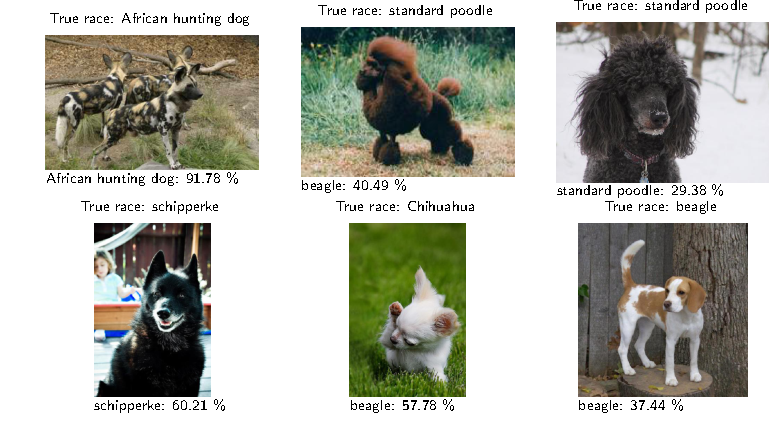
\includegraphics[width = \textwidth]{../../final_data/MiniNN_n5/visualize_predictions.pdf}
\caption{Beispielhafte Klassifizierung des Testdatensatzes mit \textsc{MiniDogNN}.
        Die Prozentzahl unter jedem Bild gibt die Wahrscheinlichkeit für die Klassenzugehörigkeit an.}
\label{fig:klasifizierung_MiniDogNN}
\end{figure}
In der Konfusionmatrix \ref{fig:MiniDogNN_Konfusionmatrix} hat sich gezeigt, dass
die Rasse \emph{Schipperke} oft mit der Rasse \emph{Afircan Hunting Dog} verwechselt
wird. Dies könnte auf die Ähnlichkeit der Schnauzenform erklärt werden. Desweiteren
können die Schwierigkeiten mit der \emph{Beagle} und \emph{Chihuahua} Klassifizierung
durch die Fellfarbe erklärt werden. Insbesondere beim kleinen Datensatz kann dies,
auf Grund der geringeren Statistik, eine große Auswirkung haben. Über diesen Ansatz
könnte auch die schlechte Klassifizierung der \emph{Poodle} Rasse erklärt werden.
Die Rassen \emph{Schippwerke} und \emph{Afircan Hunting Dog} besitzen wie die
\emph{Poodle} Rasse oftmals dunkeles Fell. Das Fell des \emph{Poodles} unterscheidt sich jedoch
in der Struktur, was eventuell von dem \textsc{MiniDogNN}-CNN nicht, aber von dem
\textsc{PreDogNN} als Feature festgestellt werden konnte.

Die Motivation für dieses Projekt war es, einen Klassifizier zu erstellen
der besser ist, als der durchschnittliche TU Dortmund Physikstudierende.
Es lässt sich zusammenfassen, dass lediglich die \textsc{PreBigDogNN}-Architektur
einen Physikstudierenden mit deutlich schlagen würde. In Verbindung mit
der formulierten Hypothese wird deutlich, dass die \textsc{PreBigDogNN}-Architektur
einem Physikstudierenden der TU Dortmund überlegen ist und eventuell als Hilfsmittel
in betracht gezogen werden sollte.

\subsection{Ausblick}
Abschließend soll noch ein Ausblick über mögliche Verbesserung gegeben werden.
Wie bereits in der Diskussion erwähnt könnte sich die Bildgröße, bis zu einer
gewissen Größe, signifikant auf die Bildgröße auswirken. Momentan ist das
Framework hierdurch die Beschaffenheit von \textsc{numpy.arrays} beschränkt.
Jedoch könnte die Verwendung von \textsc{python} \textsc{dictonaries} eine Lösung sein,
da einzelne Einträge nicht die gleiche Shape benötigen. Darüberhinaus sollte mittels
HPO die optimalen Hyperparameter für die vortranierten Modelle ermittelten werden.
Die Performance der vortranierten Modelle könnte weiterhin auch durch die Anpassung
des FCN verbessert werden. Eine letzte Möglichkeit die Genauigkeit zu erhöhen,
wäre den Datensatz eigenständig zu erweitern.

Autoencoder Bildgröße anpassen
\newpage
